\documentclass{beamer}
\usepackage{graphicx}
\usepackage{listings}
\usepackage{pgfplots}
\usepackage{pgfplotstable}
\usepackage{mathtools}
\usepackage{tikz}

\usetikzlibrary{patterns,shapes,positioning,calc}
\setbeamertemplate{bibliography item}[text]
\lstset{language=C, basicstyle=\ttfamily\scriptsize, columns=flexible, belowskip=0pt, aboveskip=0pt}

\title{Measurement Bias from Address Aliasing}

\author[Lars Kirkholt Melhus, Rune Erlend Jensen]
{Lars Kirkholt Melhus \and Rune Erlend Jensen}
\institute{
  Dept. of Computer and Information Science\\
  Norwegian University of Science and Technology \\
  Trondheim, Norway
}

\date[2016] % (optional)
{International Workshop on Automatic Performance Tuning, Chicago, May 2016}

\subject{Computer Science}

% Allocated to each presentation: 30 mins. Probably 20 mins + questions,
% a couple of minutes per slide should mean around 10 slides at the most.

\begin{document}

\frame{\titlepage}

\begin{frame}

\frametitle{Outline}

\begin{itemize}
  \item What is measurement bias?
  \item What is address aliasing?
  \item How does this help?
\end{itemize}

\end{frame}


\begin{frame}[fragile, allowframebreaks]
\frametitle{Measurement Bias}

% Show example code and plot from Mytkowitz.

\begin{itemize}
  \item Runtime performance change from external factors
  \begin{itemize}
    \item Environment variables
    \item Link ordering
  \end{itemize}
  \item Challenge for performance analysis
\end{itemize}

\begin{figure}
  \begin{lstlisting}[frame=single, xleftmargin=.01\textwidth, xrightmargin=.01\textwidth]
static int i, j, k;

int main() {
    int g = 0, inc = 1;
    for (; g < 65536; g++) {
        i += inc;
        j += inc;
        k += inc;
    }
    return 0;
}
  \end{lstlisting}
  \caption{\label{fig:microkernel}Microkernel first presented by Mytkowicz \emph{et al.}\cite{Mytkowicz:2009:WrongData}, showing bias to environment size.}
\end{figure}

% Also an optimization problem (relevant for auto-tuning).

What is the execution time of this function?

\pgfplotstableread{bin/microkernel-cycles-haswell.dat}{\stackoffsettable}
\begin{figure}
  \begin{tikzpicture}
    \begin{axis}[
        width = \textwidth,
        height = 5.0cm,
        font = \footnotesize,
        xlabel=Bytes added to environment,
        ylabel=Cycles,
        domain = 0:8192,
        xtick = {0,1024,...,8192},
        xmin = 0,
        xmax = 8192,
        cycle list name = exotic
      ]
      \addplot[ycomb] table[x expr = \thisrowno{0}*16, y = cycles:u] \stackoffsettable ;
    \end{axis}
  \end{tikzpicture}
  \caption{Measured average of 10 cycle count samples for 512 different environments; offseting stack by multiples of 16 bytes.}
\end{figure}

% Also an optimization problem (relevant for auto-tuning).

\end{frame}


\begin{frame}
\frametitle{4K Address Aliasing}

\begin{columns}[T] % align columns
\begin{column}{.48\textwidth}

\begin{itemize}
  %\item Collisions between static and automatic variables, depending on alignment of stack.
  \item Address of i, j and k are fixed for all environments.
  \item Address of g and inc is pushed down with length of environment variables.
  \item Spike when inc is at 0x7fffffffe03c + $ k \times $ 0x1000, \emph{aliasing} with i in the last 12 bits.
  \item Performance impact from \emph{false dependencies} in CPU out of order execution.
  \item Effect known as \emph{address aliasing}.
\end{itemize}

\end{column}
\hfill
\begin{column}{.48\textwidth}

% Virtual memory/randomization illustration
\begin{figure}
  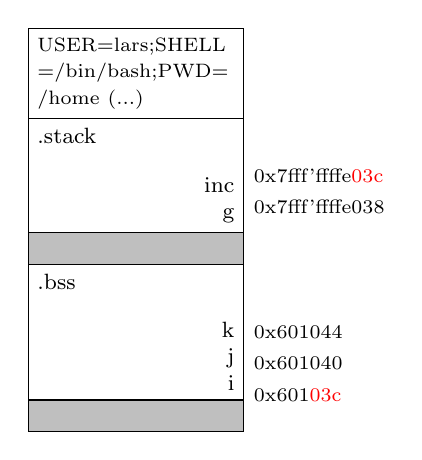
\begin{tikzpicture}[font=\footnotesize]
    % See page 453 in pgf manual
    \node [
      rectangle split, rectangle split parts=5, 
      rectangle split part fill={white, white, lightgray, white, lightgray},
      draw, anchor=center, text width=2.5cm
    ] (m) {
      \nodepart{one}
        \scriptsize{USER=lars;SHELL
        =/bin/bash;PWD=
        /home (...)}
      \nodepart{two}
        .stack
        \begin{flushright}
        inc \\
        g
        \end{flushright}
      \nodepart{four}
        .bss
        \begin{flushright}
        k \\
        j \\
        i
        \end{flushright}
    };

    \node[right, yshift=0cm] at (m.two east) {
      \scriptsize{0x7fff'ffffe{\color{red}03c}} % inc
    };
    \node[right, yshift=-0.4cm] at (m.two east) {
      \scriptsize{0x7fff'ffffe038} % g
    };

    \node[right, yshift=0cm] at (m.four east) {
      \scriptsize{0x601044} % k
    };
    \node[right, yshift=-0.4cm] at (m.four east) {
      \scriptsize{0x601040} % j
    };
    \node[right, yshift=-0.8cm] at (m.four east) {
      \scriptsize{0x601{\color{red}03c}} % i
    };

    %\draw [decorate, decoration={brace, amplitude=5pt}] (m.south west) -- (m.seven split west) 
    %  node [black, midway, xshift=-1.5cm, text width=2.0cm] 
    %    { Program code and static data } ;
    
    %\node[right] at (m.north east) { \scriptsize{0x7fff'ffffffff} } ;
    %\node[right] at (m.south east) { \scriptsize{0x400000} } ;
  \end{tikzpicture}
  \caption{4K address aliasing between stack and static data.}
\end{figure}

% Note: Could have gotten more collisions if g also was colliding with something,
%       but not noticeable effect on cycles executed.

\end{column}
\end{columns}

\end{frame}


% More generic on methodology? Not necessary for presentation maybe..
% Just to straight to the juice.
\begin{frame}
  \frametitle{How to Measure Address Aliasing}
  \framesubtitle{Using Hardware Performance Counters}

  % Some points on hardware perf counters.
  \begin{itemize}
    \item Control execution environment (disable ASLR).
    \item Using processor-specific instrumentation, we can \emph{count} various low-level events during execution.
      \begin{itemize}
        \item Cycles executed, branch prediction misses, instructions fetched, etc.
      \end{itemize}
    %\item Intel manual lists hundreds of events.
  \end{itemize}

  Events covering 4K aliasing:

  \begin{description}
    \item[{\small LD\_BLOCKS\_PARTIAL.ADDRESS\_ALIAS.}] 
    \emph{``Counts the number of loads that have partial address match with preceding stores, causing the load to be reissued.''} 
    \cite[B.3.4.4]{OptimizationManual}
  \end{description}
  %This event is listed in the manual for microarchitectures going back to ``Nehalem'', including ``Ivy Bridge'' and ``Haswell'' CPUs~\cite{Volume3B}.
  %Older architectures such as Core do not have this particular event listed, but 4K aliasing is covered by a more general event:
  \begin{description}
    \item[{\small LOAD\_BLOCKS.OVERLAP\_STORE.}] 
    \emph{``Loads that partially overlap an earlier store, or 4-Kbyte aliased with a previous store.''} 
    \cite[Table 19-17]{Volume3B}
  \end{description}

  % Describe LD_BLOCKS_PARTIAL.ADDRESS_ALIAS
\end{frame}


  % After this, done with method for detecting alias, and answers question
  % from old paper. Now lets see what else can be discovered.

  \begin{frame}
    \frametitle{Bias in Heap Allocation}

    \begin{itemize}
      \item Alias conflicts can happen between any sections of memory.
      \item While stack addresses depend on environment, heap addresses depend on allocators.
    \end{itemize}

    Looked at several allocators:

    \begin{itemize}
      \item ptmalloc (glibc)
      \item tcmalloc (Google)
      \item jemalloc
      \item Hoard
    \end{itemize}

    % Motivation for looking: Determines addresses.

    % Short survay, most use mmap for large allocations.

    % punchline: mmap always alias.

  \end{frame}

\begin{frame}[fragile]
  \frametitle{mmap}

    Most allocators use anonymous memory mapping for large allocations.

\begin{lstlisting}[frame=single, xleftmargin=.01\textwidth, xrightmargin=.01\textwidth]
$ man mmap

(...) on Linux, the mapping will be created at a nearby page boundary.
The address of the new mapping is returned as the result of the call.

\end{lstlisting}

\end{frame}

\begin{frame}[fragile]
  \frametitle{Optimization Resistant Code}

% Image of sliding window with buffers in and out (Color variables?)

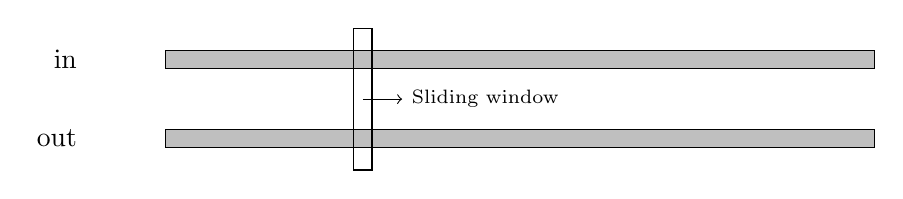
\begin{tikzpicture}[
  barstyle/.style={rectangle,fill=lightgray,draw,anchor=center,minimum width=9cm}
]
\node [barstyle] (in) at (0,1) { } ;
\node [barstyle] (out) at (0,0) { } ;
\node [rectangle,draw,minimum height=1.8cm] (bar) at (-2,0.5) { } ;

\node[] (input label) [left=of in] { in } ;
\node[] (output label) [left=of out] { out } ;

\draw[->] (-2,0.5) -- (-1.5,0.5) node [right,align=center] {\scriptsize{Sliding window}} ;

\end{tikzpicture}

% Convolution example code
\begin{figure}[t]
  \lstinputlisting[
    language=C,
    frame=single,
    xleftmargin=.00\textwidth,
    xrightmargin=.00\textwidth
  ]{bin/convolution-kernel.c}
  \caption{Simplified implementation of convolution with a fixed kernel. This program is highly sensitive to aliasing between input and output arrays, continuously generating false dependencies.}
  \label{lst:conv}
\end{figure}


    % Plots for O2 and O3

    % Manual offset code (?)

\end{frame}

  \begin{frame}
    \frametitle{Aliasing in BLAS libraries}

    % Maybe mention FFTW results from Master's?

  \end{frame}


\begin{frame}

\frametitle{References}

\scriptsize{\bibliographystyle{IEEEtran}}
\bibliography{references}

\end{frame}

\end{document}
